\chapter{System Design and Implementation Methodology}

The development of an autonomous surveillance system requires a systematic approach that integrates sensing, decision-making, actuation, and communication into a unified framework. The design of the proposed system is guided by performance requirements such as real-time detection, accuracy in targeting, and reliable long-range communication. This chapter elaborates on the design specifications, analytical modeling, system architecture, and implementation methodology adopted to achieve a functional and efficient surveillance system.

\section{Specifications for the Design}

The design of the system is driven by both functional and operational requirements. These specifications ensure that the system performs reliably under defined conditions.

\subsection{Functional Requirements}

\begin{itemize}
\item The system must continuously monitor the environment within a defined angular range.
\item It must detect objects within a specified distance threshold.
\item The system should differentiate between authorized and unauthorized entities.
\item It must generate alerts and communicate them wirelessly over long distances.
\end{itemize}

\subsection{Operational Specifications}

\begin{itemize}
\item Detection range: up to 30 cm (current prototype)
\item Angular scanning range: 0° to 180°
\item Communication range: up to several kilometers using LoRa
\item Power supply: regulated DC supply for embedded operation
\end{itemize}

These specifications form the basis for selecting components and designing system behavior.

\section{Pre-analysis and System Modeling}

Before implementation, the system is analyzed as a combination of interacting subsystems. Each subsystem is modeled based on its input-output behavior.

\subsection{Detection Model}

The ultrasonic sensor is modeled as a time-of-flight measurement system. The relationship between time and distance is given by:

\[
d = \frac{v \times t}{2}
\]

where:
\begin{itemize}
\item $d$ is distance
\item $v$ is speed of sound
\item $t$ is echo time
\end{itemize}

This model assumes constant environmental conditions and negligible noise.

\subsection{Actuation Model}

Servo motors are modeled as position-controlled systems where the output angle is proportional to the PWM signal. The mapping between pulse width and angle is linear within the operating range.

\subsection{Communication Model}

LoRa communication is modeled as a low-power wireless transmission system with parameters such as spreading factor, bandwidth, and coding rate affecting range and reliability.

\section{System Architecture}

The system architecture is modular and consists of the following primary components:

\begin{itemize}
\item Sensing Unit (Ultrasonic Sensor)
\item Processing Unit (Microcontroller)
\item Actuation Unit (Servo Motors)
\item Identification Unit (RFID)
\item Communication Unit (LoRa Module)
\end{itemize}

\begin{figure}[H]
\centering
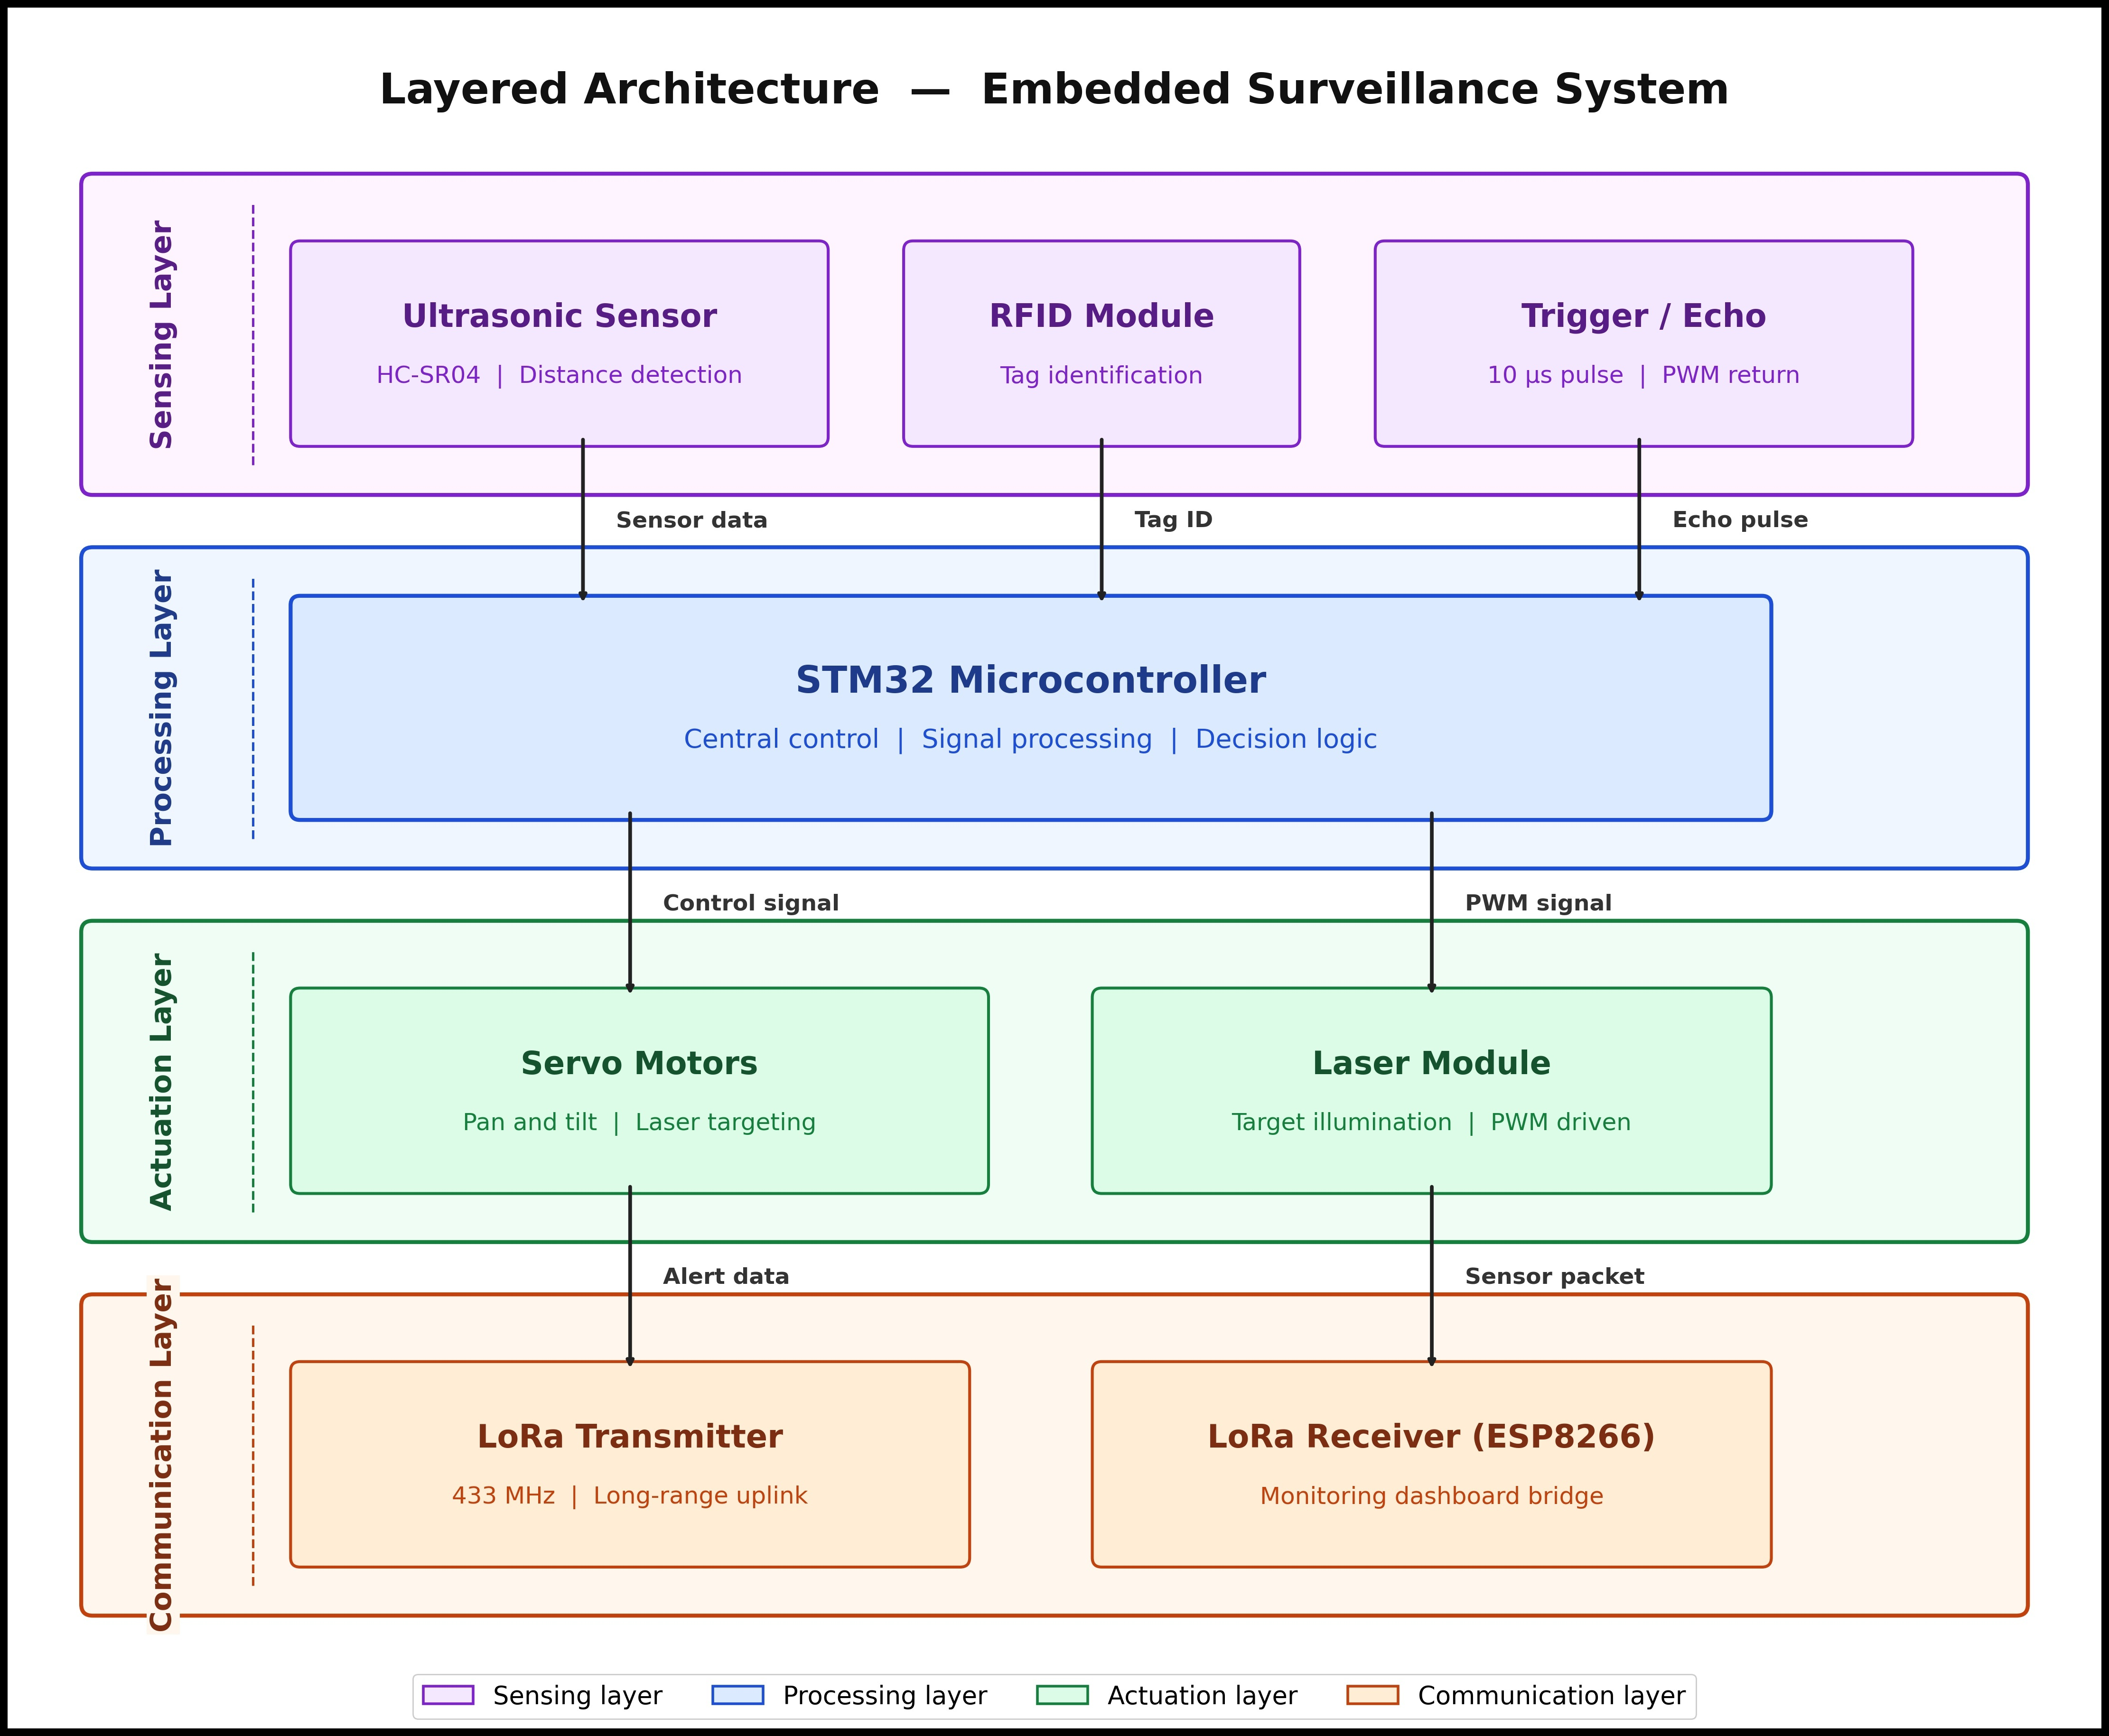
\includegraphics[width=0.75\textwidth]{figure/3.1.jpg}
\caption{Overall architecture of the autonomous surveillance system}
\label{fig:arch}
\end{figure}

Each module interacts with the central controller, forming a closed-loop system capable of autonomous operation.

\section{Design Methodology}

The design methodology follows a sequential and iterative approach to ensure reliability and accuracy.

\begin{figure}[H]
\centering
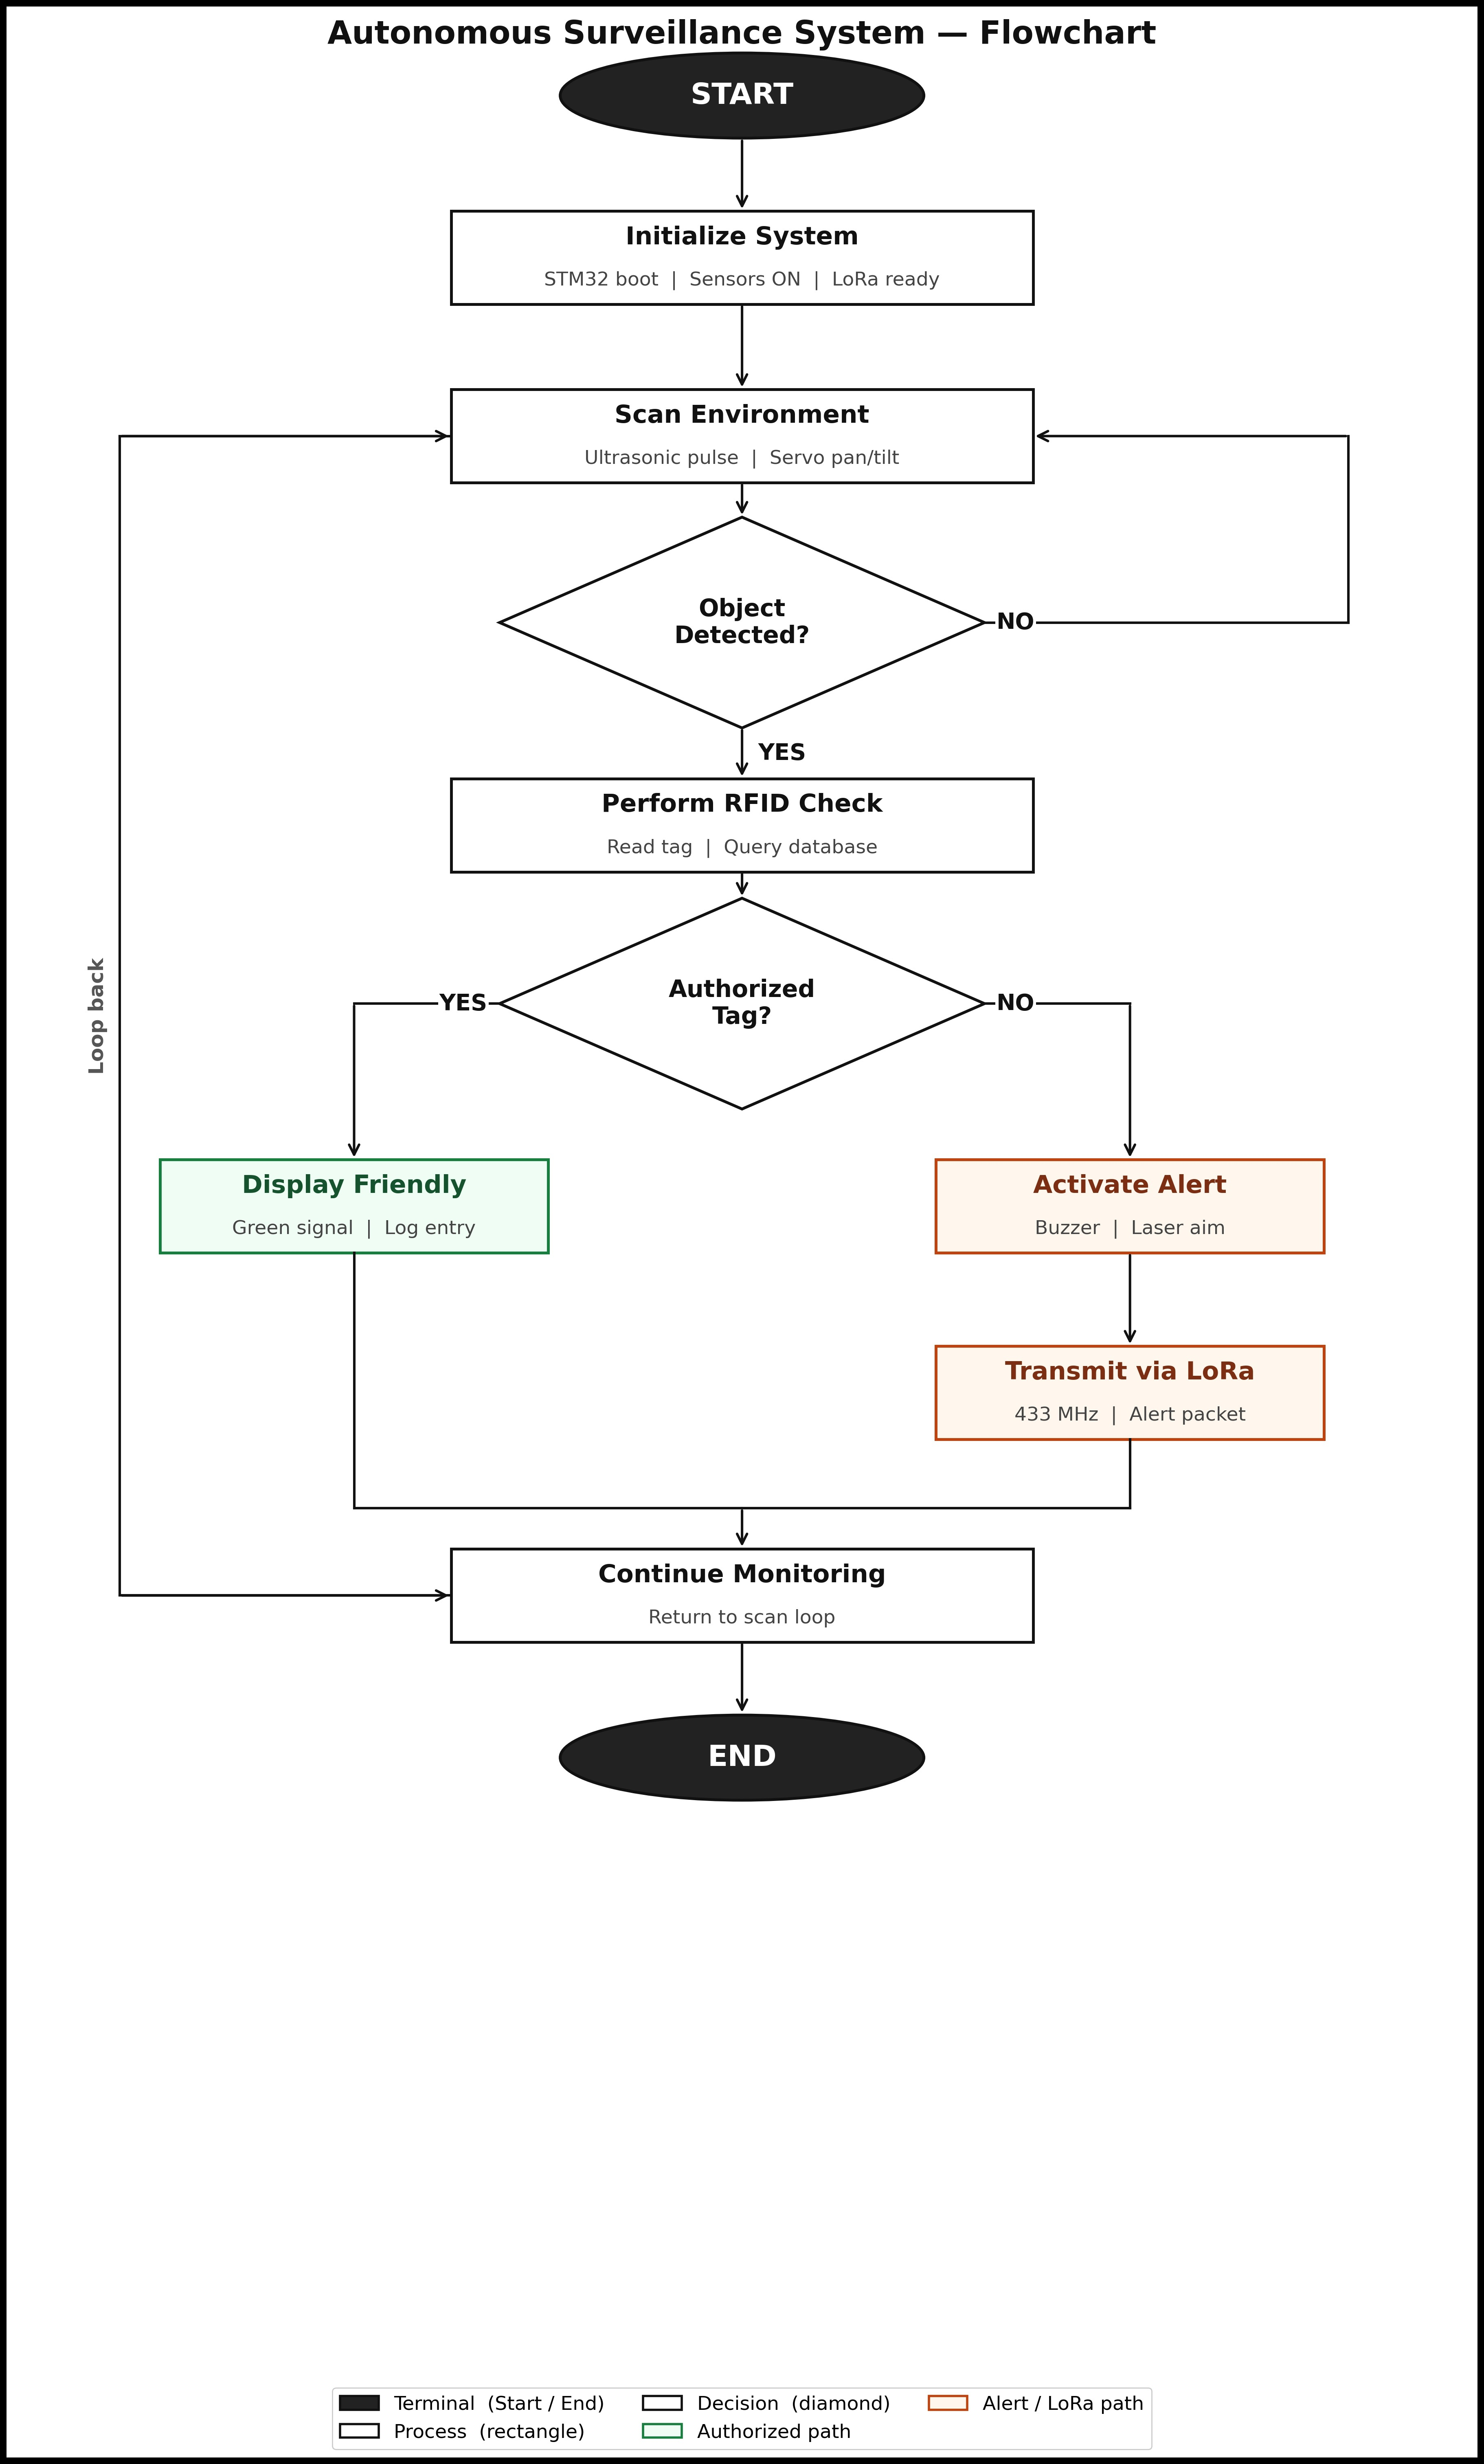
\includegraphics[width=0.7\textwidth]{figure/3.2.jpg}
\caption{Flowchart representing system operation and decision making}
\label{fig:flow}
\end{figure}

\subsection{Step 1: Environment Scanning}

The ultrasonic sensor is mounted on a servo motor which sweeps across a predefined angular range. This allows continuous monitoring of the surroundings.

\begin{figure}[H]
\centering
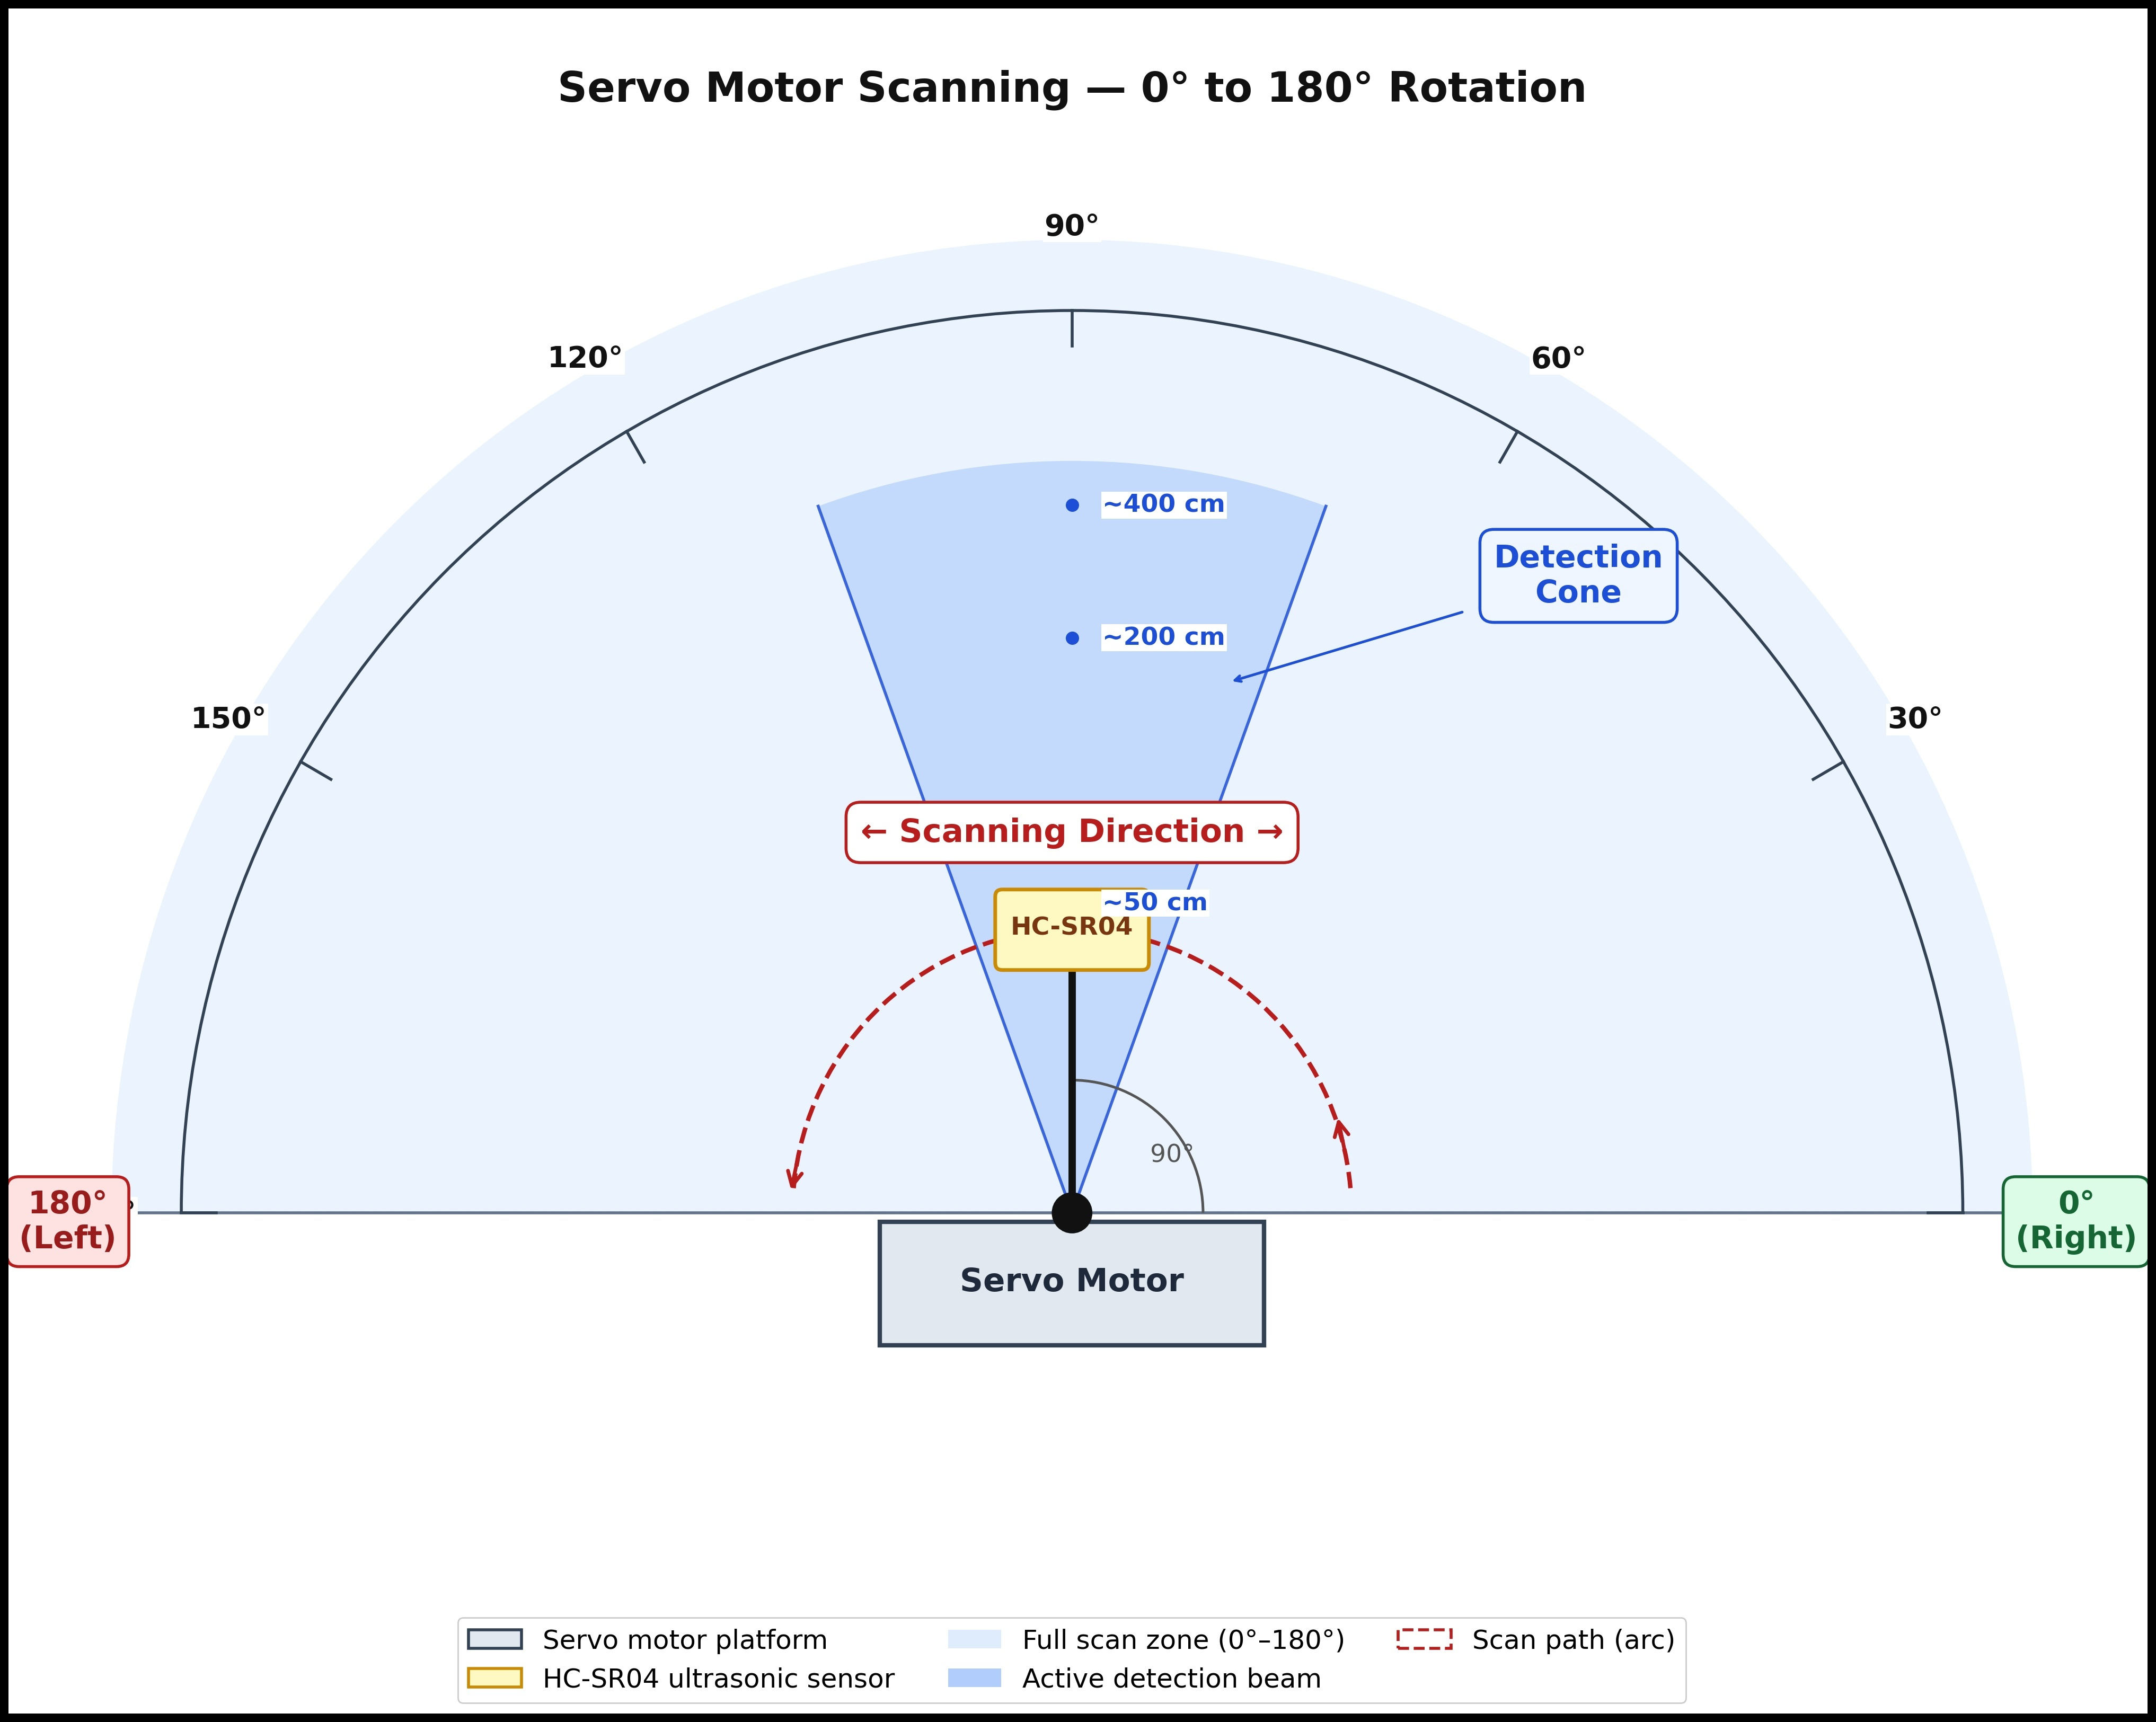
\includegraphics[width=0.65\textwidth]{figure/3.3.jpg}
\caption{Scanning mechanism using servo-mounted ultrasonic sensor}
\label{fig:scan}
\end{figure}

\subsection{Step 2: Target Detection}

At each angular position, the sensor measures distance. If the measured distance falls below the threshold, a potential target is detected.

\subsection{Step 3: Target Localization}

Once a target is detected, geometric relationships are used to calculate its position relative to the system. This enables accurate alignment of the laser.

\subsection{Step 4: Identification}

RFID technology is used to determine whether the detected entity is authorized. This step is crucial for avoiding false alarms.

\subsection{Step 5: Response Generation}

If the entity is unauthorized, the system activates the alert mechanism and transmits the information using LoRa communication.

\begin{figure}[H]
\centering
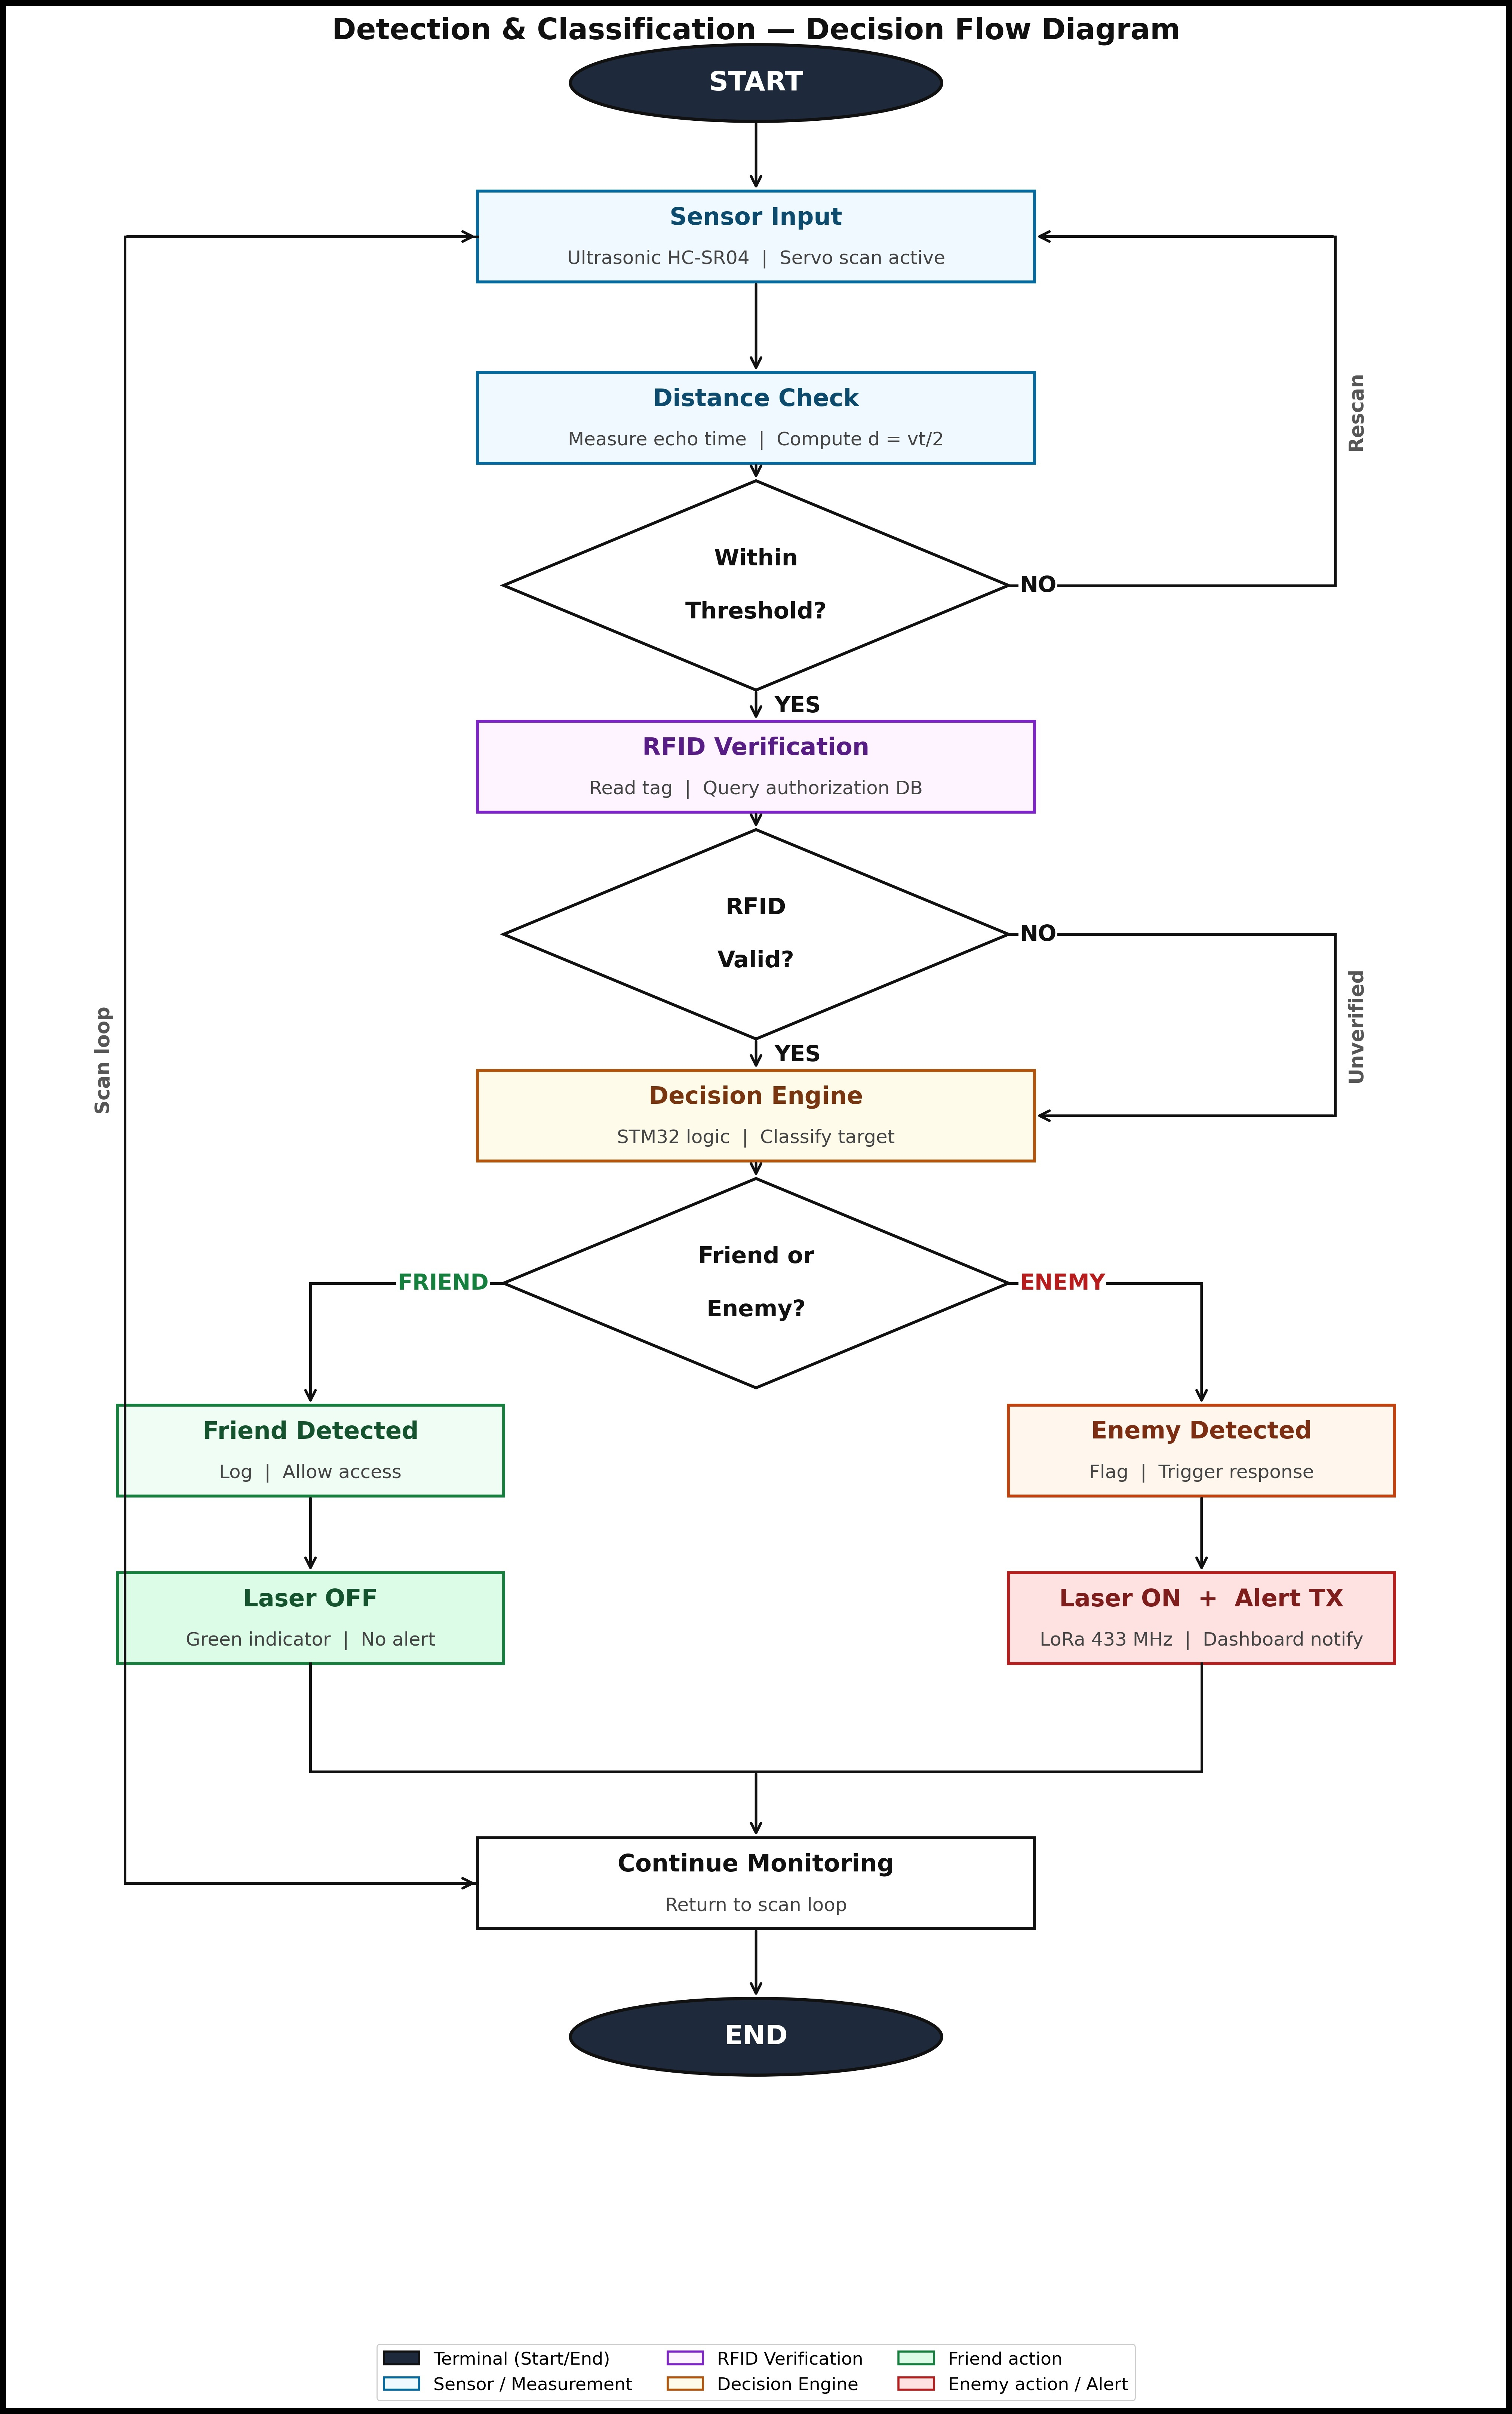
\includegraphics[width=0.7\textwidth]{figure/3.4.jpg}
\caption{Target detection and decision-making process}
\label{fig:decision}
\end{figure}

\section{Design Equations}

The mathematical formulation plays a crucial role in ensuring accurate targeting.

\subsection{Distance Calculation}

\[
\text{Distance (cm)} = \text{Time} \times 0.017
\]

\subsection{Geometric Targeting}

Using the cosine rule:

\[
b = \sqrt{a^2 + c^2 - 2ac \cos(\theta)}
\]

\[
\cos(B) = \frac{a^2 + b^2 - c^2}{2ab}
\]

\[
B = \cos^{-1}(\cdot)
\]

These equations are used to compute the required angle for precise alignment of the targeting mechanism.

\section{Experimental Techniques}

The system implementation involves several experimental techniques to ensure accuracy and reliability.

\subsection{Calibration}

Sensors and actuators are calibrated to ensure accurate measurements and positioning.

\subsection{Noise Reduction}

Filtering techniques are applied to eliminate erroneous sensor readings.

\subsection{Timing Optimization}

Precise timing control is implemented using hardware timers to ensure accurate measurements.

\section{System Integration Strategy}

Integration of multiple modules is achieved through synchronized operation controlled by the microcontroller.

\begin{itemize}
\item Sensor provides input data
\item Controller processes data
\item Actuator performs movement
\item Communication module transmits alerts
\end{itemize}

This coordinated operation ensures seamless functioning of the system.

\section{Implementation Considerations}

Several practical considerations are taken into account:

\begin{itemize}
\item Power consumption optimization
\item Hardware limitations
\item Real-time constraints
\item Environmental factors
\end{itemize}

These factors influence the design and performance of the system.

\section{Chapter Summary}

This chapter presented the detailed design methodology and analytical foundation of the autonomous border surveillance system. The specifications, system modeling, architectural design, and mathematical formulations were discussed to provide a comprehensive understanding of the system implementation. The next chapter focuses on the practical implementation and results obtained from the developed system.